%=======================02-713 LaTeX template, following the 15-210 template==================
%
% You don't need to use LaTeX or this template, but you must turn your homework in as
% a typeset PDF somehow.
%
% How to use:
%    1. Update your information in section "A" below
%    2. Write your answers in section "B" below. Precede answers for all 
%       parts of a question with the command "\question{n}{desc}" where n is
%       the question number and "desc" is a short, one-line description of 
%       the problem. There is no need to restate the problem.
%    3. If a question has multiple parts, precede the answer to part x with the
%       command "\part{x}".
%    4. If a problem asks you to design an algorithm, use the commands
%       \algorithm, \correctness, \runtime to precede your discussion of the 
%       description of the algorithm, its correctness, and its running time, respectively.
%    5. You can include graphics by using the command \includegraphics{FILENAME}
%
\documentclass[11pt]{article}
\usepackage{amsmath,amssymb,amsthm}
\usepackage{graphicx}
\usepackage[margin=1in]{geometry}
\usepackage{fancyhdr}
\usepackage{listings}
\usepackage{float} 
\usepackage{subfig}

\setlength{\parindent}{0pt}
\setlength{\parskip}{5pt plus 1pt}
\setlength{\headheight}{13.6pt}
\newcommand\question[2]{\vspace{.25in}\hrule\textbf{#1: #2}\vspace{.5em}\hrule\vspace{.10in}}
\renewcommand\part[1]{\vspace{.10in}\textbf{(#1)}}
\newcommand\algorithm{\vspace{.10in}\textbf{Algorithm: }}
\newcommand\correctness{\vspace{.10in}\textbf{Output: }}
\newcommand\runtime{\vspace{.10in}\textbf{Running time: }}
\pagestyle{fancyplain}
\lhead{\textbf{\NAME\ (\ANDREWID)}}
\chead{\textbf{Project\HWNUM}}
\rhead{\today}
\begin{document}\raggedright
%Section A==============Change the values below to match your information==================
\newcommand\NAME{Yao Xiao}  % your name
\newcommand\ANDREWID{2019180015}     % your andrew id
\newcommand\HWNUM{2}              % the homework number
%Section B==============Put your answers to the questions below here=======================

% no need to restate the problem --- the graders know which problem is which,
% but replacing "The First Problem" with a short phrase will help you remember
% which problem this is when you read over your homeworks to study.

\question{1}{Programming 2} 

\part{a} \algorithm The implement of PKDF2 and AES-GCM
\begin{lstlisting}
import javax.crypto.*;
import javax.crypto.spec.GCMParameterSpec;
import javax.crypto.spec.PBEKeySpec;
import javax.crypto.spec.SecretKeySpec;
import java.security.*;
import java.security.spec.InvalidKeySpecException;
import java.security.spec.KeySpec;
import java.util.Base64;

public Cryptogram(String psd) {

    String password = psd;

    if (password == null || password.isEmpty()) {
        KeyGenerator keyGen = KeyGenerator.getInstance("AES");
        // choose aes-256
        keyGen.init(256);
        password = Base64.getEncoder().encodeToString(keyGen.generateKey().getEncoded());
    }

    final byte[] salt = new byte[64];
    random = SecureRandom.getInstanceStrong();
    random.nextBytes(salt);

    // use PKDF2 to derive the secret K
    SecretKeyFactory secretKeyFactory = SecretKeyFactory.getInstance("PBKDF2WithHmacSHA512");
    KeySpec passwordBasedEncryptionKeySpec = new PBEKeySpec(password.toCharArray(), salt, 10000, 256);
    SecretKey secretKeyFromPBKDF2 = secretKeyFactory.generateSecret(passwordBasedEncryptionKeySpec);
    this.mSecretKey = new SecretKeySpec(secretKeyFromPBKDF2.getEncoded(), "AES");
    this.mCipher = Cipher.getInstance("AES/GCM/NoPadding");
}

public byte[] encrypt(byte[] data){
    byte[] nonce = new byte[32];
    random.nextBytes(nonce);
    mGCMParameterSpec = new GCMParameterSpec(16 * 8, nonce);
    mCipher.init(Cipher.ENCRYPT_MODE, mSecretKey, mGCMParameterSpec);
    return mCipher.doFinal(data);
}

public byte[] decrypt(byte[] data) {
    mCipher.init(Cipher.DECRYPT_MODE, mSecretKey, mGCMParameterSpec);
    return mCipher.doFinal(data);
}

\end{lstlisting}

\part{b} \algorithm The implement of Client
\begin{lstlisting}
import java.net.ServerSocket;
import java.net.Socket;

public void listen() {
    this.localServerSocket = new ServerSocket(this.localPort);
    System.out.println("local listening port: " + serverAddr + ":" + serverPort);
    while (true) {
        try {
            Socket mSocket = localServerSocket.accept();
            new ClientThread(this.serverAddr, this.serverPort, mSocket, this, this.pw).start();
            } catch (Exception e) {
                e.printStackTrace();
        }
    }
}
\end{lstlisting}

\part{c} \algorithm The implement of Server
\begin{lstlisting}
public void listen() {
    System.out.println("server listening port: " + port);
    serverSocket = new ServerSocket(port);
    while (true) {
        try {
            Socket mSocket = serverSocket.accept();
            new ServerThread(mSocket, this, this.pw).start();
        }
    } catch (Exception e) {
        e.printStackTrace();
    }
}
\end{lstlisting}



\part{d} \correctness

\begin{figure}[H]
    \centering
    \subfloat{
        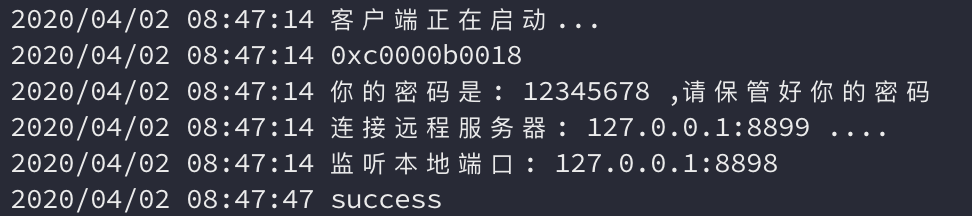
\includegraphics[width=0.45\textwidth]{f1}}
    \subfloat{
        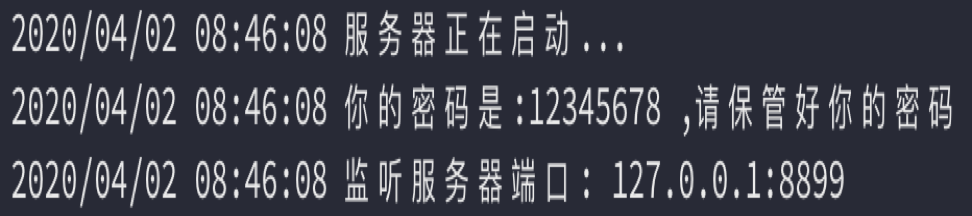
\includegraphics[width=0.45\textwidth]{f2}}
    \caption{Client and Server}
\end{figure}
\begin{figure}[H]
    \centering
    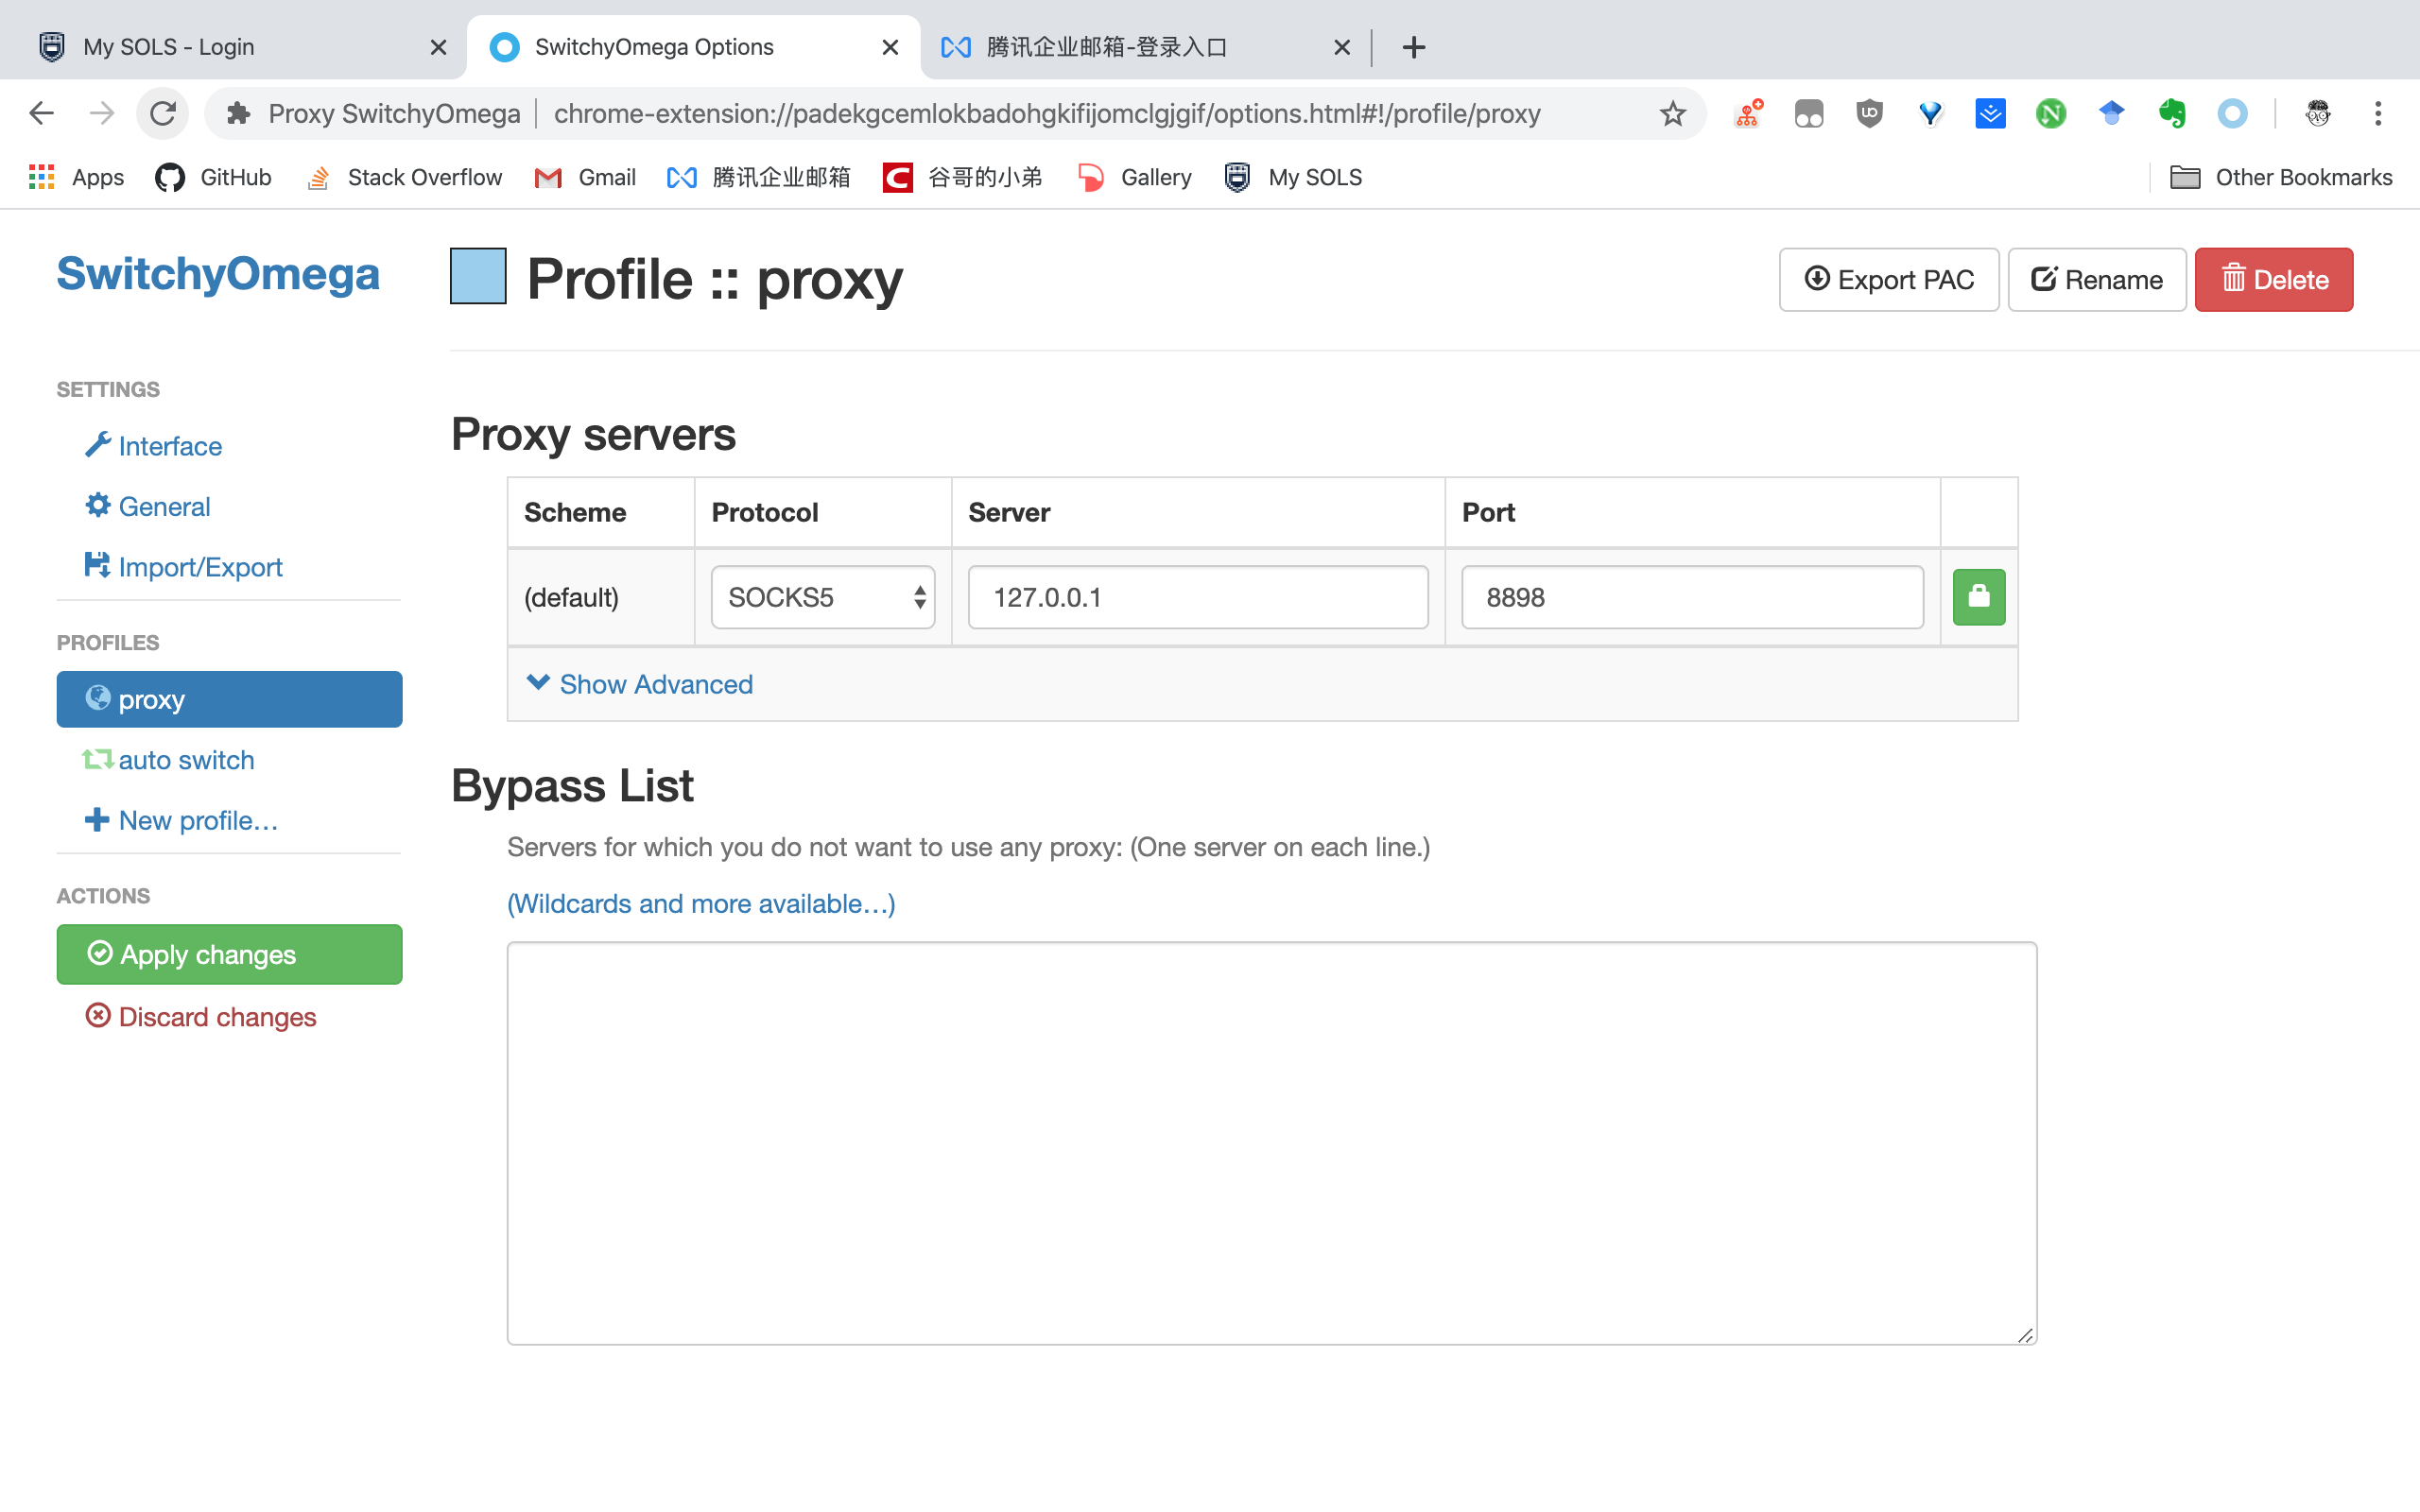
\includegraphics[width=0.8\textwidth]{s5}
    \caption{Socks5Proxy}
\end{figure}
\begin{figure}[H]
    \centering
    \subfloat{
        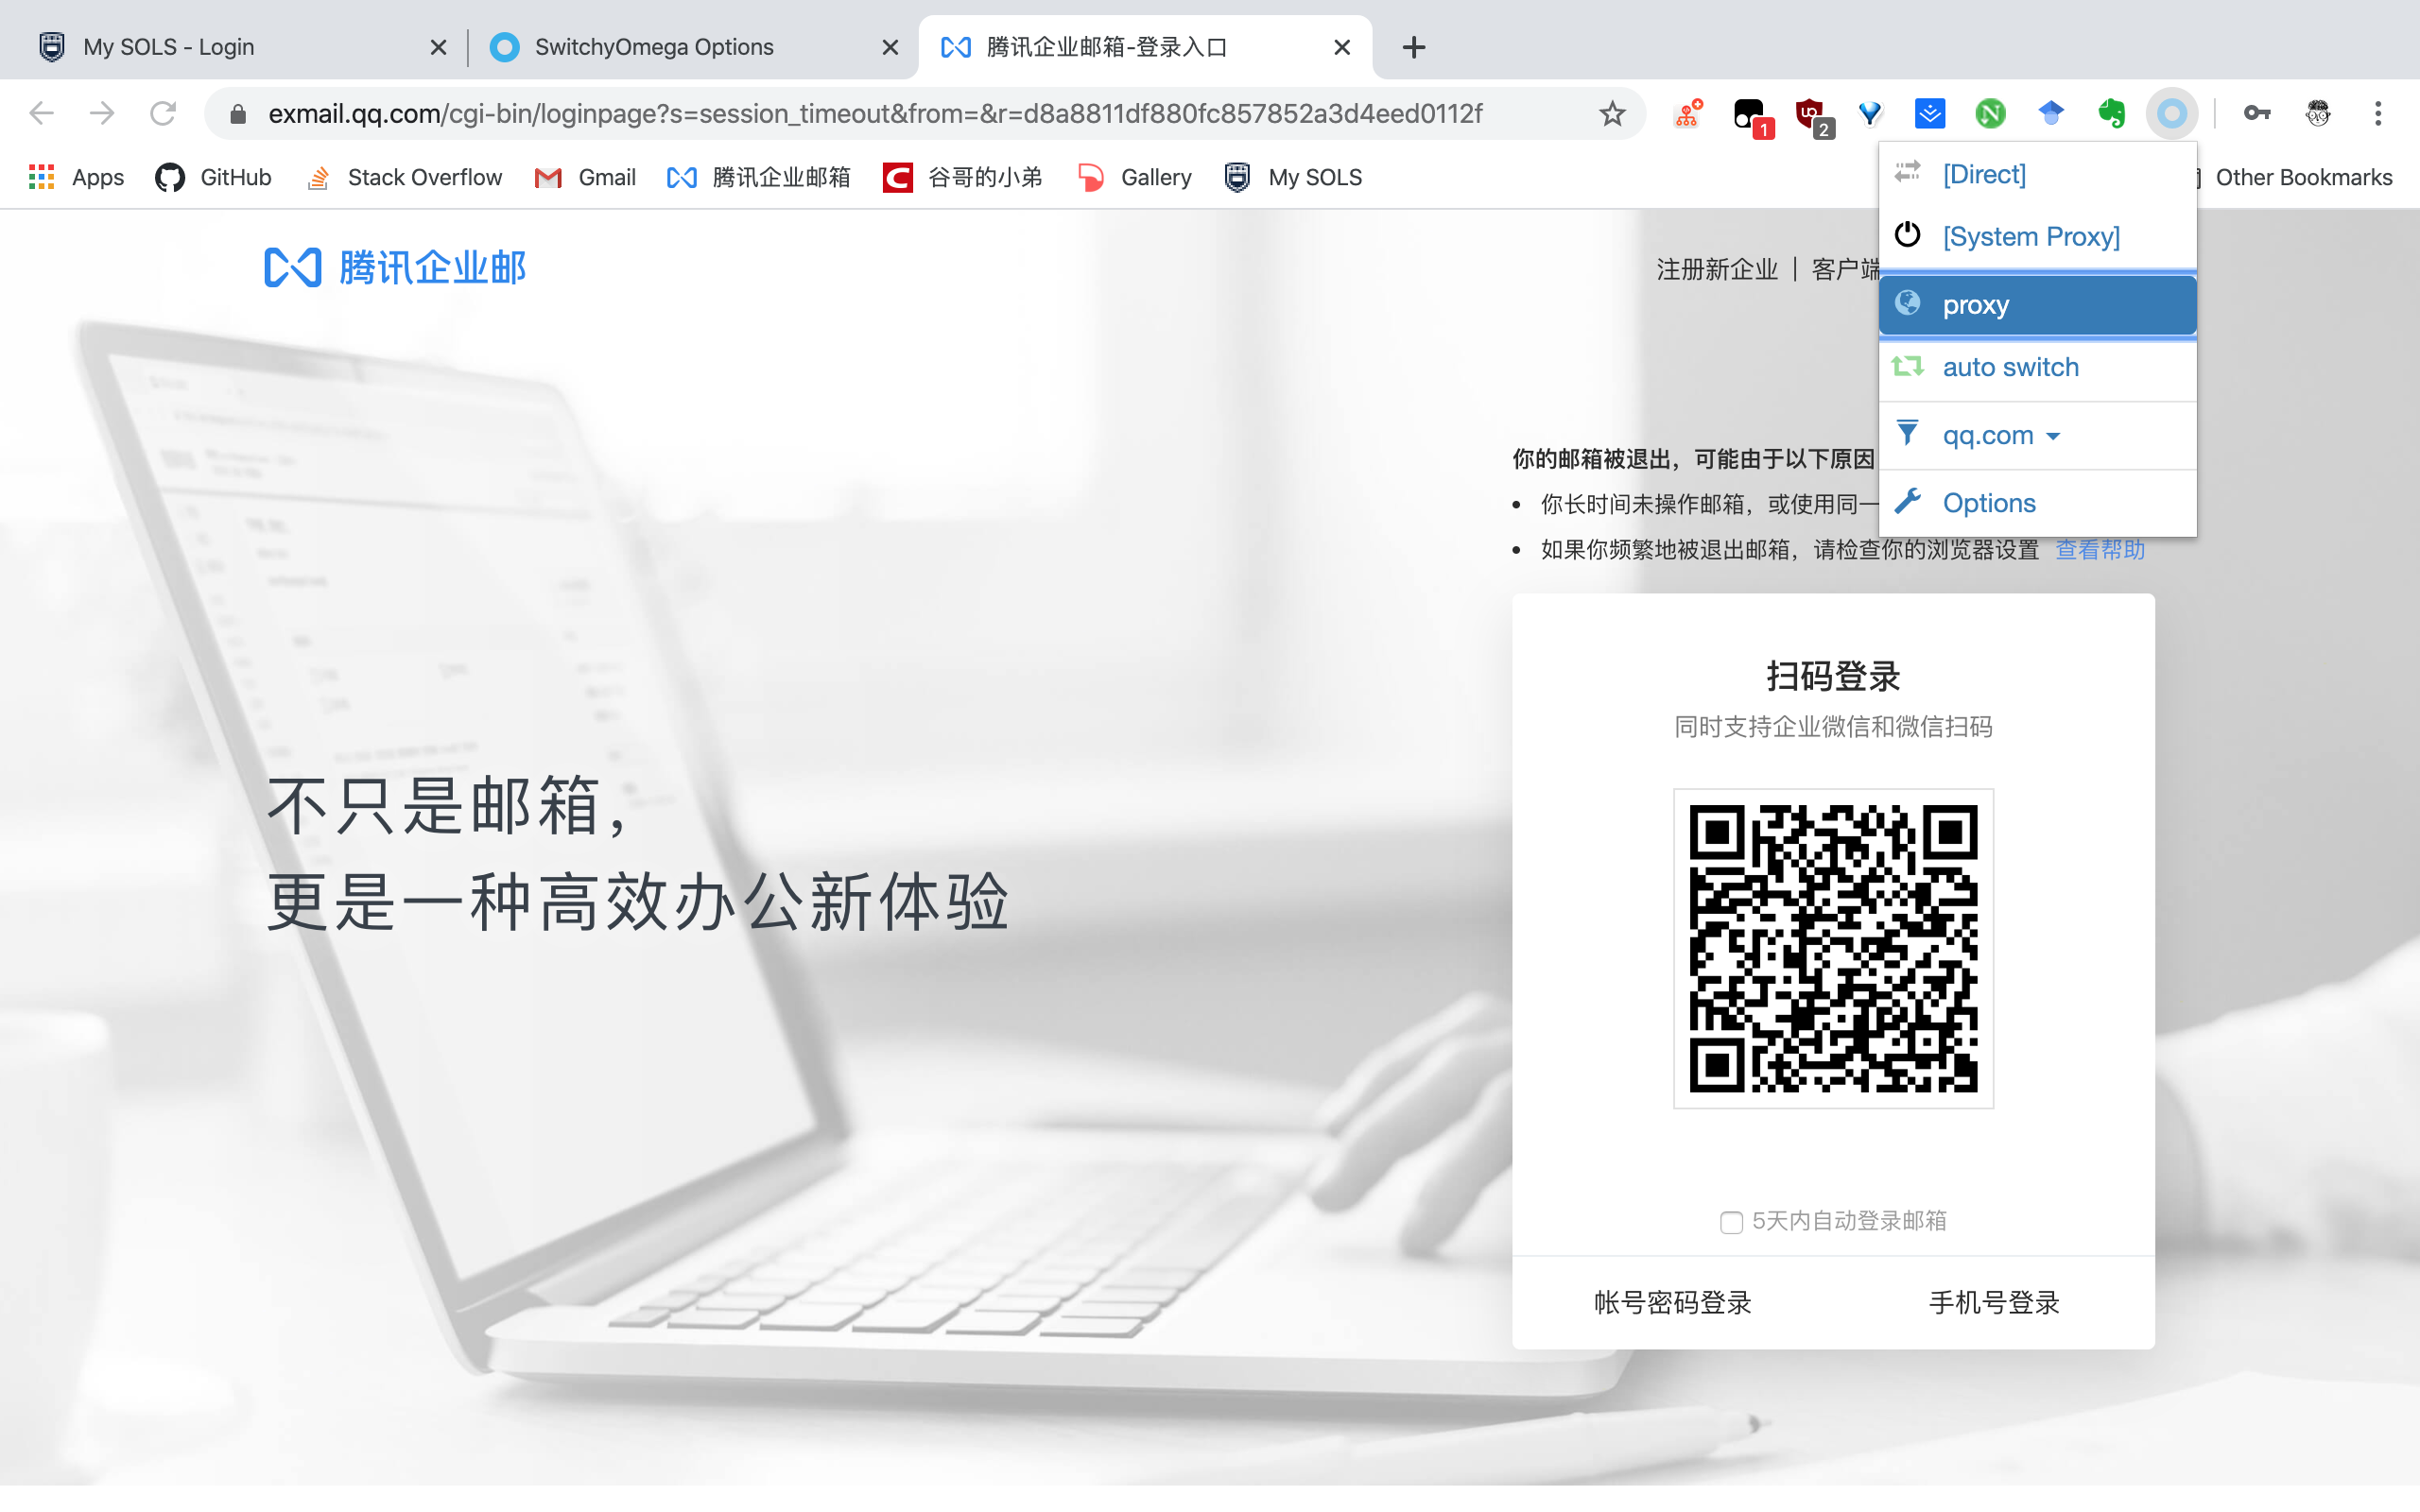
\includegraphics[width=0.45\textwidth]{chrome}}
    \subfloat{
        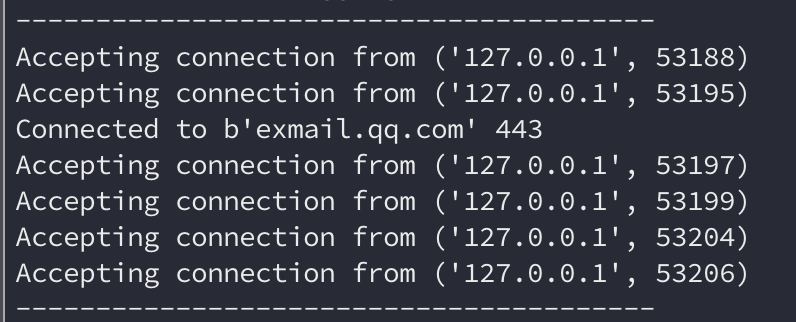
\includegraphics[width=0.45\textwidth]{email}}
    \caption{Output}
\end{figure}



\end{document}
